


\section{Segments and segment computers}

  \begin{frame}<beamer>
    \frametitle{Plan}
    \tableofcontents[sectionstyle=show/shaded]
  \end{frame}

\begin{frame}
  \frametitle{Segments}
 

   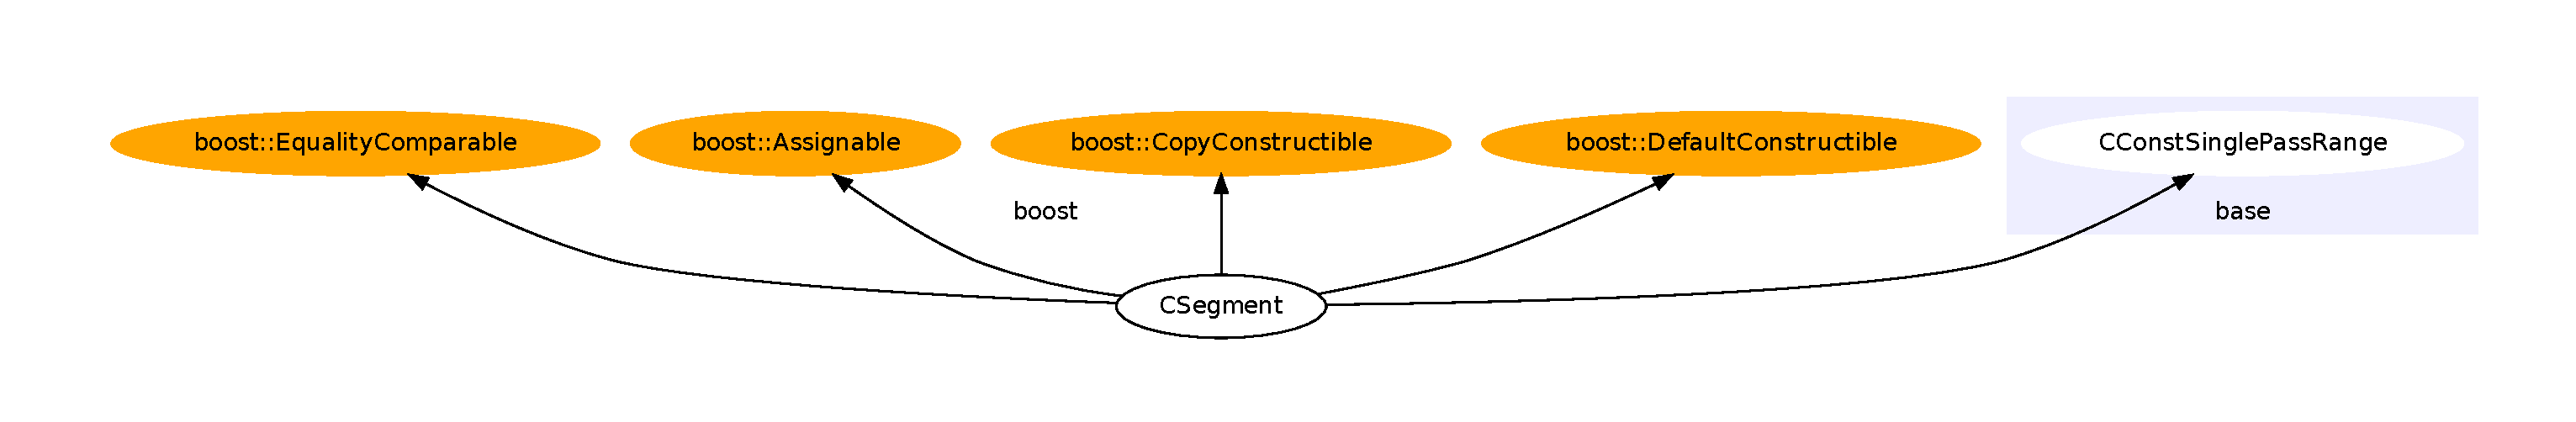
\includegraphics[width=1\textwidth]{segmentGraph}

  \begin{block}{Segment}
It is a valid and \emph{not empty} range. 

~

Type:
\begin{itemize}
  \item ConstIterator: at least a model of a \emph{bidirectional} iterator
\end{itemize}

Main methods:
\begin{itemize}
  \item begin(): begin iterator of the range
  \item end(): end iterator of the range (past-the-end)
\end{itemize}

Invariant: ( begin() != end() )
  \end{block}

\end{frame}

\begin{frame}
  \frametitle{The detection problem}
 
  \begin{block}{Class of segments $\Sigma_P$}
Set of segments such that for each segment of the set, 
a given predicate $P$ is true: 

$\forall s \in \Sigma_P,  P(s) = \text{true}$ 
  \end{block}

  \begin{block}{Detection problem}
Deciding whether a given segment 
belongs to a class of segments or not:  

is $s \in \Sigma_P$ ? or equivalently is $P(s)$ true ? 
  \end{block}

  \begin{block}{Segment computer}
Segment that can 
\begin{enumerate}
 \item constructs other instances of its own type
 \item control its own extension so that the predicate $P$ remains true
\end{enumerate}
  \end{block}

\end{frame}

\begin{frame}
  \frametitle{Segment computers}
 

 \begin{center}
   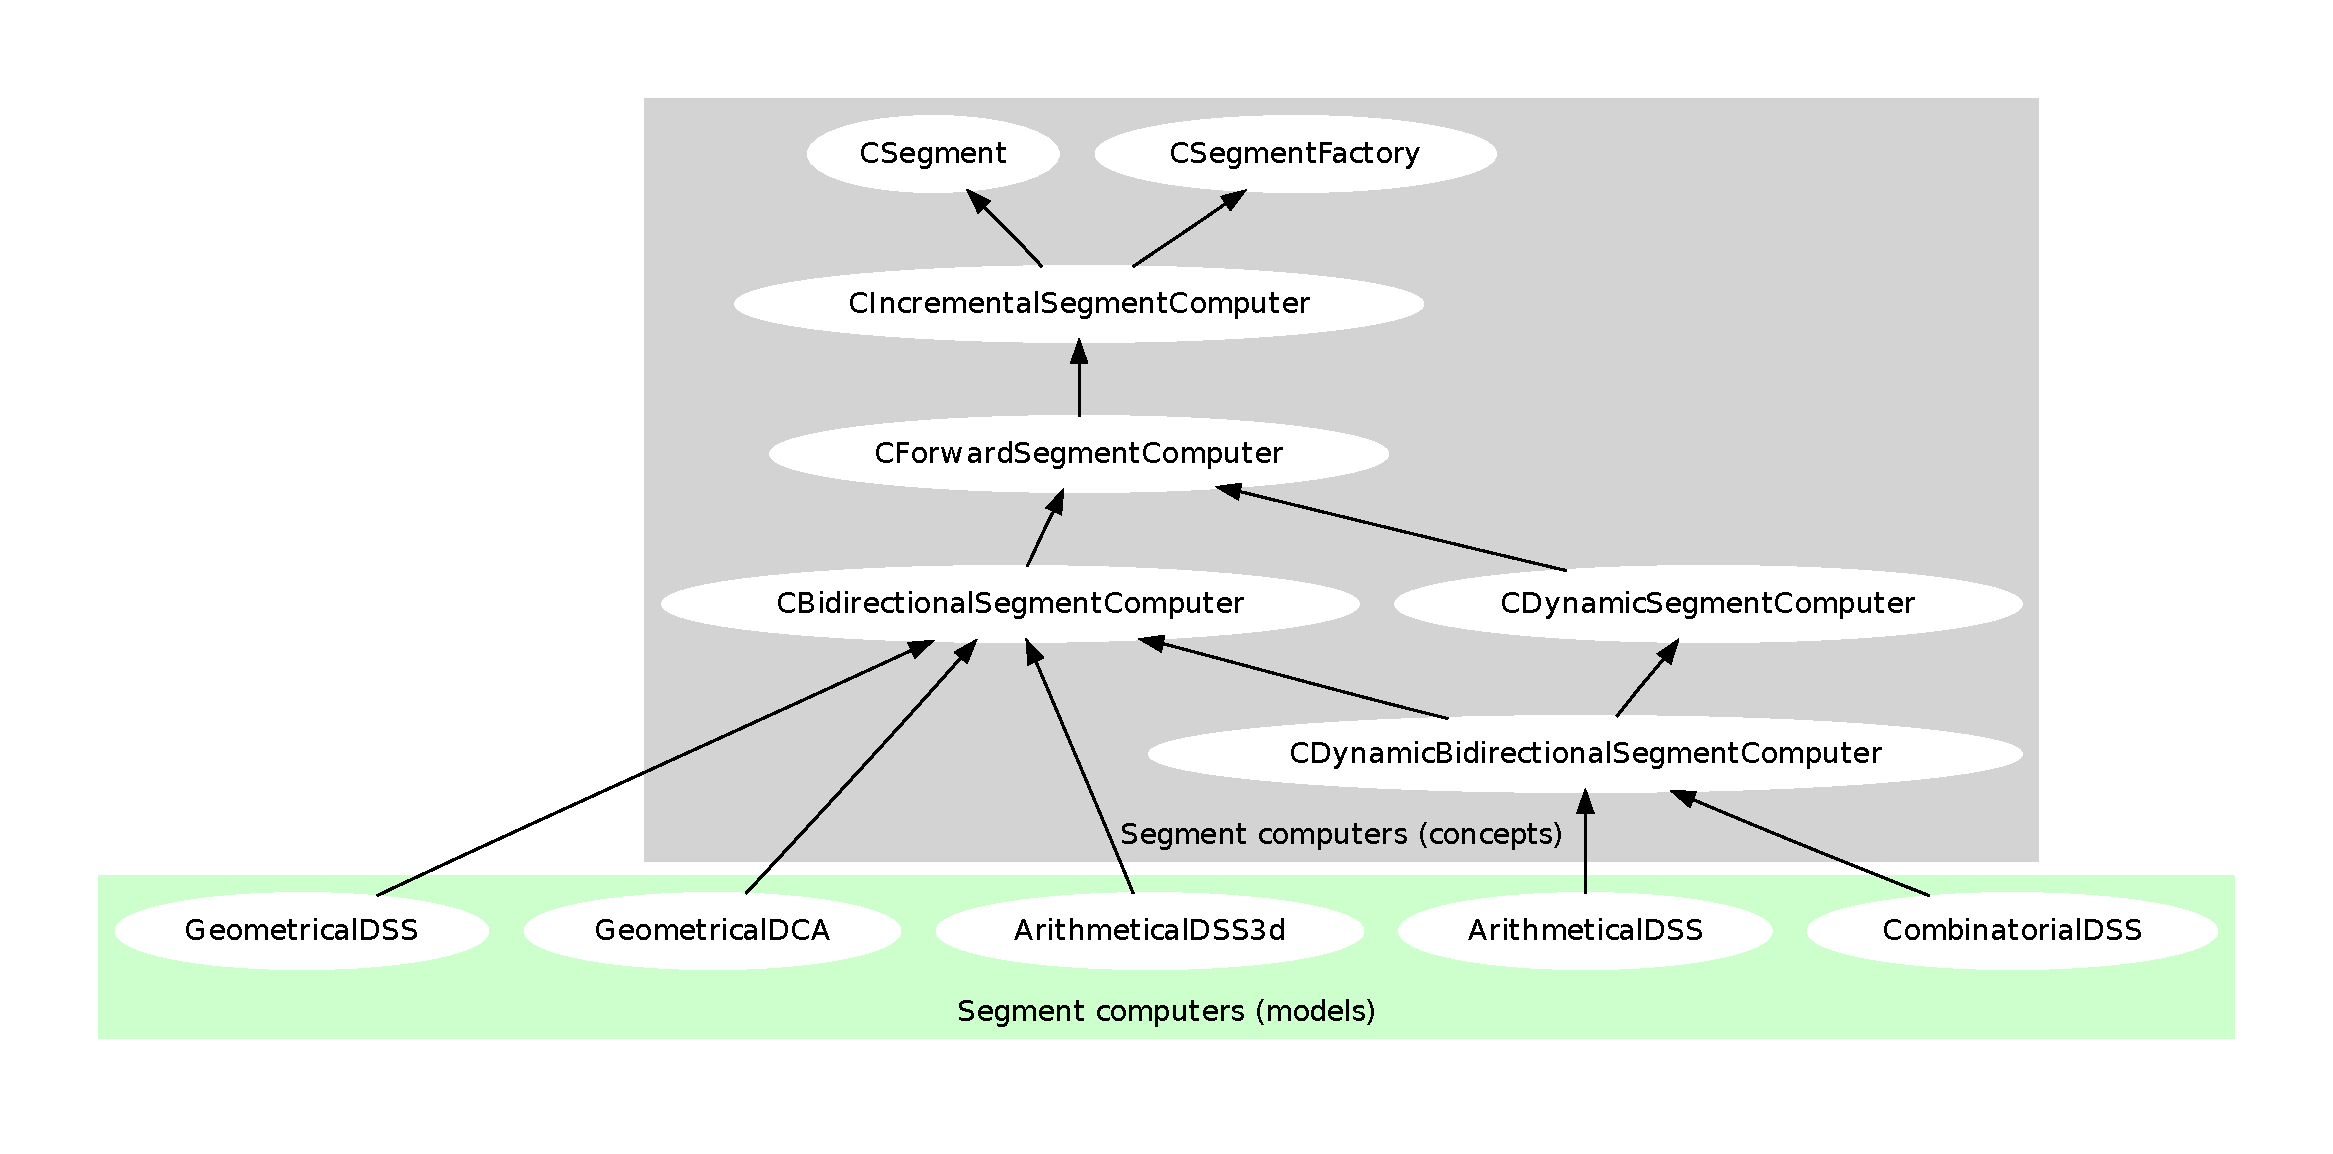
\includegraphics[width=1\textwidth]{segmentComputersGraph}
 \end{center}

\end{frame}

\begin{frame}[containsverbatim,fragile]
  \frametitle{CIncrementalSegmentComputer: syntactic constraints}

Refinement of CSegment and CSegmentFactory that provides in addition the following methods:
\begin{itemize}
 \item void init ( const ConstIterator\& it ) : set the segment to the element pointed by it.
 \item bool isExtendable () : return 'true' if the segment can be extended to the element pointed by end() and 'false' otherwise (no extension is performed).
 \item bool extend () : return 'true' and extend the segment to the element pointed by end() if it is possible, return 'false' and does not extend the segment otherwise.
\end{itemize}

~

Detection of a segment:
  \begin{lstlisting}
    //s is a segment computer
    //[begin,end) is a range
    s.init( begin );
    while ( (s.end() != end) && (s.extend()) ) {} 
  \end{lstlisting}

Avoiding infinite loops with circulators:
  \begin{lstlisting}
    //s is a segment computer
    //c is a circulator
    s.init( c );
    while ( (s.end() != s.begin()) && (s.extend()) ) {}
  \end{lstlisting}

\end{frame}

%incremtal vs forward
\begin{frame}[containsverbatim,fragile]
  \frametitle{CIncrementalSegmentComputer vs CForwardSegmentComputer}

Same syntactic constraints but different semantic constraints

~

Models of CIncrementalSegmentComputer verify: 
  \begin{lstlisting}
for ( ConstIterator it = s.begin(), 
      ConstIterator itEnd = s.end();
      it != itEnd; ++it)
  { // [s.begin(), it) is a segment:
    s.init( s.begin() ); 
    bool flag = true; 
    while ( (s.end() != it)&&(flag) ) { flag = s.extend(); }
    ASSERT( flag ); 
  }
  \end{lstlisting}

In addition, models of CForwardSegmentComputer verify: 
  \begin{lstlisting}
for ( ConstIterator it = s.begin(), 
      ConstIterator itEnd = s.end();
      it != itEnd; ++it)
  { // [it, itEnd) is a segment:
    bool flag = true; 
    while ( (s.end() != itEnd)&&(flag) ) { flag = s.extend(); }
    ASSERT( flag ); 
  }
  \end{lstlisting}

\end{frame}

\begin{frame}
  \frametitle{Useful functions}
 
The code can be different if an iterator or a circulator is used as the nested ConstIterator type. Moreover, some tasks can be made faster for a given kind of segment computer than for another kind of segment computer. Basically, 
given a maximal segment, computing the next maximal segment is faster for dynamic segment computers than for forward segment computers. That's why many generic functions are provided in SegmentComputerUtils.h:

\begin{itemize}
 \item maximalExtension, oppositeEndMaximalExtension, maximalSymmetricExtension,
 \item maximalRetraction, oppositeEndMaximalRetraction,
 \item longestSegment (init the segment computer),
 \item firstMaximalSegment, lastMaximalSegment, mostCenteredMaximalSegment,
 \item previousMaximalSegment, nextMaximalSegment,
\end{itemize}



\end{frame}


